\chapter{Theoretical Background} % Main chapter title
\label{chap:Chapter2} % For referencing the chapter elsewhere, use \ref{Chapter1} 
\epigraph{''Let no one ignorant of geometry enter” }{\textit{Plato}}

O χώρος των \hyperref[abbr:WSN]{WSN} έχει και αυτός τα τελευταία χρόνια υψηλό ερευνητικό ενδιαφέρον.
Θα μπορούσε να πει κανείς - λόγο το ότι αποτελεί ένα πιο γενικό κλάδο - περισσότερο από ότι αυτό των 
drones. Συνεπώς θα μεταφερθούμε σε πρώτο επίπεδο στο πιο γενικό φάσμα, αυτό των \hyperref[abbr:WSN]{WSN} 
για να προσεγγίσουμε το localization problem. 

Όταν μιλάμε για \hyperref[abbr:WSN]{WSN}, αναφερόμαστε σε αυτόνομα ηλεκτρονικά συστήματα, χωρικά διασκορπισμένα σε ένα πεδίο - τα οποία συχνά περιλαμβάνουν
αισθητήρες και επικοινωνούν με τα γειτονικά τους ή σταθμούς βάσης για να μεταφέρουν πληροφορία \cite{wsn-wikipedia} \cite{farooqiazam2016location}.

Το καθένα από αυτά τα ανεξάρτητα συστήματα ονομάζεται \textbf{Node}. Ενώ για το κάθε μεμονωμένο node 
μπορεί να έχουμε στην διάθεση μας location information ή όχι. 
Μία πρώτη σκέψη θα ήταν κάθε node ενός συστήματος αισθητήρων να περιλαμβάνει \hyperref[abbr:GPS]{GPS} ώστε να γνωρίζουμε 
την θέση του. Αυτό μπορεί γρήγορα να καταρριφθεί σαν σκέψη, αν αναλογιστούμε αρχικά ότι το Global Navigation Satellite System (\hyperref[abbr:GNSS]{GNSS})
δεν είναι διαθέσιμο σε κάθε περιβάλλον λειτουργίας (π.χ. εσωτερικούς χώρους), όπως επίσης μπορεί να μην είναι δυνατή η χρήση του σε όλους τους κόμβους
ενός συστήματος, λόγο περιορισμών όπως το κόστος, μέγεθος του node και energy consumption \cite{farooqiazam2016location}.   

\begin{table}[H]
    \caption{Nodes' names definitions}
    \label{tab:nodes-names-definition}
	\centering
	\resizebox{1\textwidth}{!}{
		\begin{tabular}{ll}
			\toprule
			\textbf{Node name} & \textbf{Definition}  \\
			\midrule
				Unknown/Free/Dumb/Non-anchors & Their position is unknown \\
				Beacons/Anchors/Landmarks & Nodes with known location information \\
				Settled & Initial unknown nodes with estimated position \\
			\bottomrule
		\end{tabular}
	}
\end{table}

Στην υπάρχουσα βιβλιογραφία \cite{farooqiazam2016location} \cite{wsn-Localization-systems} \cite{wsn-Localization-techniques} βρίσκουμε ότι
nodes των οποίων η θέση είναι γνωστή ή άμεσα υπολογίσιμη, συχνά ονομάζονται \textbf{Beacons}. Πληροφορία σχετικά με την θέση αυτών
των nodes είναι γνωστή, είτε γιατί έχουν τοποθετηθεί από εμάς σε προκαθορισμένες θέσεις, είτε μέσου ενός εξωτερικού συστήματος
όπως το \hyperref[abbr:GPS]{GPS} \cite{angle-of-arrival}.
Αντίθετα κόμβοι για τους οποίους δεν έχουμε αρχικά πληροφορία της θέσης τους, ονομάζονται \textbf{Non-anchors}.
Άλλος ένας σημαντικός ορισμός, που θα πρέπει να αναφερθεί είναι ότι συχνά ονομάζουμε \textbf{Settle} nodes, 
αυτά τα οποία αρχικά δεν γνωρίζαμε την θέση τους αλλά στην συνέχεια την εκτιμήσαμε.
Στο Table \ref{tab:nodes-names-definition} παρουσιάζονται συνοπτικά τα διάφορα ονόματα που έχουν δοθεί ανά 
καιρούς για το κάθε τύπο node.

Σκοπός ενός localization system είναι, με χρήση της γνώσης που έχουμε για τα beacon nodes να εκτιμήσουμε
την θέση όσο περισσότερων unknown nodes ώστε να τα μετατρέψουμε σε settled nodes και η εκτίμηση της κάθε
θέσης να είναι με όσο το δυνατόν μικρότερο error απόκλισης. 

\begin{figure} [H]
	\centering
	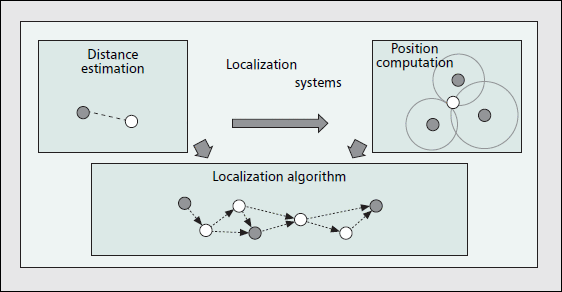
\includegraphics[scale=0.5]{Images/Theoretical-Background/localization-systems-components.png}
	\decoRule
	\caption[Localization System components]{Localization System components based on \cite{wsn-Localization-systems} (\href{https://ieeexplore.ieee.org/document/4407221}{URL})}
	\label{fig:Localization-Systems-components}
\end{figure}

Οι συγγραφείς του \cite{wsn-Localization-systems} επιχειρούν να χωρίσουν ένα localization system, ώστε 
αυτό να αποτελείται από τρία διακριτά components, αυτή τη κατηγοριοποίηση την υιοθετούν κατά την έρευνα τους και οι ερευνητές του \cite{localization-systems-components}. Πρώτο μπορεί να θεωρηθεί αυτό του \textbf{Distance/Angle Estimation}, 
που σκοπό έχει να υπολογίσει την απόσταση ή γωνία που έχουν δύο nodes του συστήματος μεταξύ τους.
Η πληροφορία που θα παραχθεί από αυτό το component θα χρησιμοποιηθεί στα άλλα μέρη του συστήματος.
Στην συνέχεια υπάρχει το \textbf{Position Computation}, δουλειά του οποίου είναι να υπολογίσει την θέση ενός
node με βάση την γνώση που έχουμε για τα beacons και την πληροφορία που λάβαμε από το πρώτο component.
Ενώ τέλος είναι το κύριο μέρος του συστήματος, με όνομα \textbf{Localization Algorithm} και ουσιαστικά είναι
ο προκαθορισμένος τρόπος που θα ακολουθηθεί για να υπολογιστεί η θέση των unknown nodes με βάση όλες τις 
πληροφορίες που έχουμε.
Στο Figure \ref{fig:Localization-Systems-components} δίνεται η απεικόνιση που έδωσαν οι συγγραφείς του 
\cite{wsn-Localization-systems} για να εξηγήσουν το παραπάνω. Ενώ στο Figure \ref{fig:Localization-system}
έχει γίνει μία προσπάθεια να κατηγοριοποιηθούν τα κομμάτια καθώς και τεχνικές των Localization Systems,
με βάση τα \cite{farooqiazam2016location} \cite{wsn-Localization-systems} \cite{wsn-Localization-techniques}
και αναλύονται στην συνέχεια του κεφαλαίου.

\begin{figure} [H]
	\tikzset{
		basic/.style  = {draw, text width=2cm, font=\sffamily},
		root/.style   = {basic, thin, align=center, fill=white, text width=5cm},
		level 1/.style = {sibling distance=16em, level distance=5em},
		level-2/.style = {basic, thin, align=center, fill=white, text width=5.5cm},
		level-31/.style = {basic, thin, align=center, fill=white, text width=2cm},
		level-32/.style = {basic, thin, align=center, fill=white, text width=2.8cm},
		level-33/.style = {basic, thin, align=center, fill=white, text width=5cm},
		level-4/.style = {basic, thin, align=center, fill=white, text width=4.5cm},
		level-42/.style = {basic, thin, align=center, fill=white, text width=4.8cm},
		edge from parent/.style={->,solid,black,thick,draw}, 
		edge from parent path={(\tikzparentnode.south) -- (\tikzchildnode.north)},
		>=latex, node distance=1.5cm, edge from parent fork down
	}
	\centering
	\resizebox{1\textwidth}{!}{
		\begin{tikzpicture}[]
			\node[root] {\textbf{Localization Systems}}
				child {node[level-2] (c1) {\textbf{Distance/Angle Estimation}}}
				child {node[level-2] (c2) {\textbf{Position Computation}}}
				child {node[level-2] (c3) {\textbf{Localization Algorithm}}};
			
			% -----------------------------------------------------------------------------
			% Distance/Angle
			\node [level-31, below of = c1, xshift=-25pt] (c11) {Distance};
				\node [level-4, below of = c11, xshift=50pt] (c111) {Received Signal Strength};
				% \node [level-4, below of = c111] (c112) {Lighthouse approach};
				\node [level-4, below of = c111] (c113) {Propagation time based measurements};
					\node [level-42, below of = c113, xshift=30pt] (c1131) {One-way propagation time};
					\node [level-42, below of = c1131] (c1132) {Roundtrip propagation time};
					\node [level-42, below of = c1132] (c1133) {Time Difference of Arrival};
					\foreach \value in {1,2,3} \draw[->] (c113.197) |- (c113\value.west);
				\foreach \value in {1,3} \draw[->] (c11.195) |- (c11\value.west);

			\node [level-31, below of = c1133, xshift=-80pt] (c12) {Angle};
				\node [level-4, below of = c12, xshift=70pt] (c121) {Receiver Antenna Amplitude response};
				\node [level-4, below of = c121] (c122) {Receiver Antenna Phase response};
				\foreach \value in {1,2} \draw[->] (c12.210) |- (c12\value.west);
			\foreach \value in {1,2}   \draw[->] (c1.188) |- (c1\value.west);
			
			% Position Computation
			\node [level-32, below of = c2, xshift=25pt] (c21) {Trilateration};
			\node [level-32, below of = c21] (c22) {Bounding box};
			\node [level-32, below of = c22] (c23) {Triangulation};
			\node [level-32, below of = c23] (c24) {Multilateration};
			\node [level-32, below of = c24] (c25) {Probabilistic approaches};
			\node [level-32, below of = c25] (c26) {Central position};
			\foreach \value in {1,...,6} \draw[->] (c2.196) |- (c2\value.west);

			% Localization Algorithm
			\node [level-33, below of = c3, xshift=10pt] (c31) {Range-based/Range-free};
			\node [level-33, below of = c31] (c32) {Distributed/Centralized \\ Position Computation};
			\node [level-33, below of = c32] (c33) {Relative/Absolute Positioning};
			\node [level-33, below of = c33] (c34) {Indoor/Outdoor scenarios};
			\node [level-33, below of = c34] (c35) {One-hop/Multihop};
			\node [level-33, below of = c35] (c36) {With/Without Infrastructure};
			\foreach \value in {1,...,6} \draw[->] (c3.187) |- (c3\value.west);
		\end{tikzpicture}
	}
	\decoRule
	\caption[Localization System overview]{Localization System overview}
	\label{fig:Localization-system}
\end{figure}

Με βάση τον παραπάνω διαχωρισμό των Localization Systems σε τρία διακριτά μέρη, μπορούμε να καταλάβουμε
ότι η απόκλιση της εκτίμησης του συνολικού συστήματος, εξαρτάται από τα σφάλματα  του κάθε μεμονωμένου μέρους.

%----------------------------------------------------------------------------------------
%	SECTION 1
%----------------------------------------------------------------------------------------
\section{Distance/Angle Estimation} \label{sec:Chapter2-1} 

\subsection{Distance}\label{sec:Chapter2-1-1}

Θα ξεκινήσουμε με μία σύντομη ανάλυση των τεχνικών εκτίμησης της απόστασης μεταξύ δύο nodes
που χρησιμοποιούνται ήδη. 

%----------------------------------------------------------------------
\subsubsection{Received Signal Strength}
Η πρώτη τεχνική η οποία έχει χρησιμοποιηθεί για τον υπολογισμό απόστασης στα 
\hyperref[abbr:WSN]{WSN}, είναι αυτή με όνομα Received Signal Strength Indicator
(\hyperref[abbr:RSSI]{RSSI}) και έχει ως αρχή την χρήση της έντασης της ισχύς ενός 
σήματος που λαμβάνουμε στον δέκτη, ως τρόπο υπολογισμού της απόστασης
του πομπό από αυτόν. Path loss ή path attenuation \cite{wikipedia-Path_loss} ονομάζεται η μείωση της ισχύς
ενός σήματος καθώς αυτό διαδίδεται.
Στον ελεύθερο χώρο η λαμβανόμενη ισχύς $P_r(d)$ που ανιχνεύει ο πομπός
μπορεί να περιγράφεται από το μοντέλο του Free Space Path Loss (\hyperref[abbr:FSPL]{FSPL}) \cite{wikipedia-fspl} και να υπολογιστεί
μέσω της Friis transmission equation \cite{wsn-Localization-techniques} \cite{rssi-wlan} \cite{wikipedia-friis-equation} - σχέση (\ref{eq:signal-strength}).

\begin{align}
	P_r(d)=\frac{P_tG_tG_r\lambda^2}{(4\pi)^2d^2} \label{eq:signal-strength}
\end{align}

Όπου $P_t$ είναι η ισχύς που στέλνει ο πομπός, $G_t$ είναι το gain της κεραίας του
πομπού, $G_r$ το gain της κεραίας του δέκτη, λ είναι το μήκος κύματος του σήματος
το οποίο μεταδίδουμε και d η απόσταση του πομπού από τον δέκτη. Αν θεωρήσουμε ότι 
τα $G_t$, $G_r$ και λ είναι μη μεταβλητές τιμές - με $C_f = \frac{G_tG_r\lambda^2}{(4\pi)^2}$ - τότε μπορούμε να καταλήξουμε
στην (\ref{eq:signal-strength-simple}) \cite{rssi-simple-formula}.

\begin{align}
	P_r(d)=C_f\frac{P_t}{d^2} \label{eq:signal-strength-simple}
\end{align}

Αυτό που μπορούμε να δούμε από την παραπάνω σχέση είναι ότι, ιδανικά στον ελεύθερο 
χώρο σε Line of Sight (\hyperref[abbr:LoS]{LoS}) μετάδοση -
η ισχύς του σήματος που λαμβάνει ο πομπός εξαρτάται από το αντίστροφο τετράγωνο της
απόστασης των δύο nodes. Η σχέση (\ref{eq:signal-strength-simple}) συχνά αναφέρεται σε watt, 
όμως όταν μιλάμε για transmitting power αντί για την χρήση των watt, είναι αρκετά βολική
η χρήση του dBm \cite{wikipedia-dBm}. Για αυτό τον λόγω παρακάτω παραπείθονται τα conversion
equations, από το ένα στο άλλο \cite{rssi-wlan} \cite{wikipedia-dBm}. 

\begin{align}
	\left\{
		\begin{array}{ll}
			P[dBm]= 10\cdot log_{10}\left(\frac{P[mW]}{1[mW]}\right) \\[10pt]
			\quad \quad P[mW] = 10^\frac{(P[dBm])}{10}
		\end{array}
	\right.
\end{align}

Ενώ το Figure \ref{fig:Ideal-RSSI-over-distance} περιγράφει σχηματικά το ιδανικό μοντέλο της εξάρτηση της ισχύς με την αύξηση
της απόστασης όταν χρησιμοποιούμε στον δέκτη μέτρηση σε dΒm. 

%-------------------------------------------

\begin{figure} [H]
	\centering
	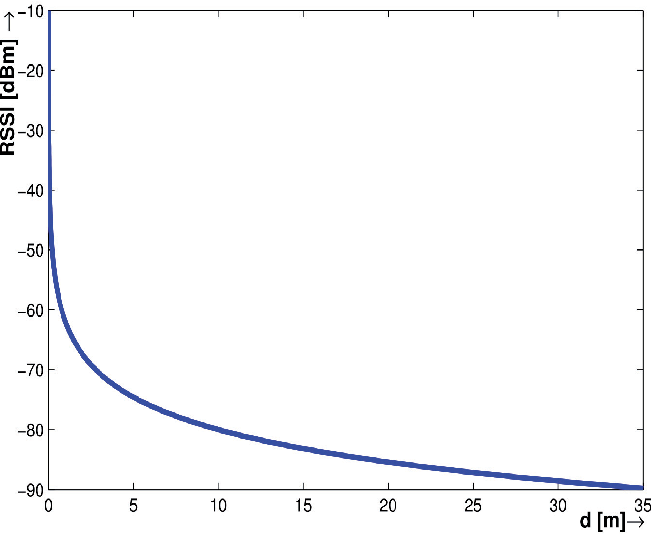
\includegraphics[scale=0.32]{Images/Theoretical-Background/Ideal-RSSI-over-distance.png}
	\decoRule
	\caption[Ideal RSSI over distance]{Ideal RSSI over distance based on \cite{ideal-rssi-model}}
	\label{fig:Ideal-RSSI-over-distance}
\end{figure}

Αν λοιπόν, μετράμε την ισχύ με την οποία λαμβάνουμε ένα σήμα, μπορούμε να είμαστε σε θέση να υπολογίσουμε την απόσταση που βρίσκεται
ο πομπός από εμάς.
Αυτή η μέθοδος παρόλο που είναι αρκετά δημοφιλής και οικονομική για τον υπολογισμό της απόστασης
- λόγω του ότι δεν απαιτεί επιπλέον αισθητήρες - σε πραγματικές 
συνθήκες αντιμετωπίζει αρκετά προβλήματα, καθώς οι μετρήσεις μπορούν να επηρεαστούν από θόρυβο,
ανακλάσεις του σήματος, διαθλάσεις, δυναμικά περιβάλλοντα ή εμπόδια σε αυτά, Non-Line of Sight (\hyperref[abbr:NLoS]{NLoS}) μετάδοση, 
ή ακόμα και errors στο hardware 
\cite{wsn-Localization-systems} \cite{ideal-rssi-model}.
Σε ένα βαθμό μπορεί να βελτιωθεί η απόδοση με στατικό ή δυναμικό calibration του συστήματος 
όμως μέχρι τώρα δεν χρησιμοποιείται για εκτίμηση απόστασης σε εφαρμογές όπου nodes έχουν μεγάλη
απόσταση μεταξύ τους ή μας ενδιαφέρει να έχουμε μεγάλη ακρίβεια προσέγγισης της απόστασης \cite{ideal-rssi-model}.

%----------------------------------------------------------------------
\subsubsection{Propagation Time}
Σε αυτήν την κατηγορία εκτίμησης απόστασης μεταξύ nodes - η οποία βασίζεται σε χρονικές μετρήσεις της διάδοσης του σήματος Time of Flight (\hyperref[abbr:ToF]{ToF})
- κατά κύριο λόγο χρησιμοποιούνται δύο βασικές τεχνικές, η Time of Arrival (\hyperref[abbr:ToA]{ToA}) και η Time 
Difference of Arrival (\hyperref[abbr:TDoA]{TDoA}) \cite{wsn-Localization-systems}. 

\begin{figure} [H]
    \centering
    % -----------------
    \begin{minipage}{.5\textwidth}
      \centering
      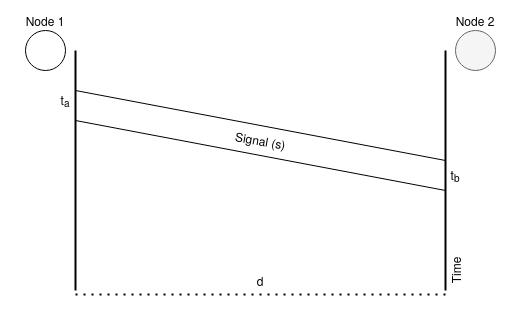
\includegraphics[width=\linewidth]{../Photos/toa-oneway.png}
      {(a) One-way}
    \end{minipage}%
    % -----------------
    \begin{minipage}{.5\textwidth}
      \centering
      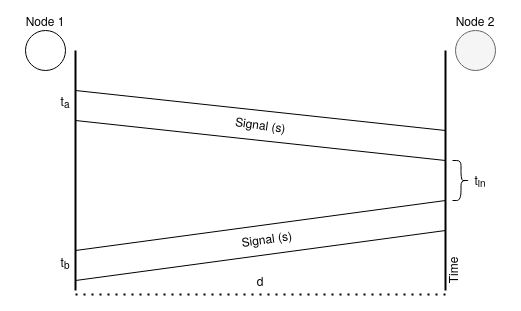
\includegraphics[width=\linewidth]{../Photos/toa-roundtrip.png}
      {(b) Roundtrip}
    \end{minipage}
    \hfill \break
    \decoRule
    \caption[Time of Arrival cases]{Time of Arrival cases}
    \label{fig:Time-of-Arrival-cases}
\end{figure}

Θα ξεκινήσουμε με μία σύντομη περιγραφή της \hyperref[abbr:ToA]{ToA}. Από την κινηματική γνωρίζουμε την 
σχέση (\ref{eq:speed}), η οποία συσχετίζει την ταχύτητα κίνησης ενός σώματος V ως το πηλίκο της μεταβολής
της θέσης $\mathrm{d}s$ - που έκανε το σώμα, προς τον χρόνο $\mathrm{d}t$ που χρειάστηκε για να πραγματοποιηθεί η μεταβολή \cite{Kinematics}.

\begin{align}
	V=&\frac{\mathrm{d}s}{\mathrm{d}t} \label{eq:speed} \\
	d=&s(t_b-t_a) \label{eq:tod-distance}
\end{align}

Αξιοποιώντας την (\ref{eq:speed}) ως αρχή, μπορούμε να καταλήξουμε στην (\ref{eq:tod-distance}) για να εκτιμήσουμε
την απόσταση d που βρίσκονται δύο nodes μεταξύ τους, αν ένα κύμα κινείται με ταχύτητα $s$ και χρειάστηκε 
χρόνο $t$ για να μεταδοθεί από το ένα node στο άλλο. Στο Figure \ref{fig:Time-of-Arrival-cases} (a) απεικονίζεται
σχηματικά αυτό, όπου $t=t_b-t_a$ με $t_b$ η χρονική στιγμή που φτάνει το κύμα στο receiver και $t_a$
η χρονική στιγμή η οποία ξεκινάει από τον transmitter. Σε περίπτωση που μιλάμε για Radio Frequency 
(\hyperref[abbr:RF]{RF}) η ταχύτητα μετάδοσης του κύματος είναι ίση με την ταχύτητα μετάδοσης του φωτός $c_o$, το οποίο 
σε $1μs$ διανύει περίπου 300m.
Με βάση αυτό, μπορούμε εύκολα να καταλάβουμε ότι για να έχουμε ακριβή αποτελέσματα είναι αρκετά σημαντικό
τα clocks των δύο nodes να είναι απόλυτα συγχρονισμένα για να μην έχουμε error απόκλισης, πράγμα που
απαιτεί να κάνουμε το συνολικό σύστημα αρκετά πιο πολύπλοκο σχεδιαστικά 
ώστε η απόκλιση μας να είναι σε ανεκτά σημεία για την εφαρμογή \cite{wsn-Localization-systems} \cite{wsn-Localization-techniques}.

Μπορούμε να το παρακάμψουμε αυτό, με το να γίνει η μέτρηση σε roundtrip μετάδοση, Figure \ref{fig:Time-of-Arrival-cases} (b).
Σε αυτήν την περίπτωση το ένα node στέλνει ένα σήμα, και μόλις το λάβει ένα γειτονικό node, απαντάει πίσω στο πρώτο. 
Με αυτόν τον τρόπο η μέτρηση του χρόνου εκκίνησης $t_a$ και άφιξης $t_b$ του σήματος γίνονται στο ίδιο node - 
άρα δεν χρειάζεται συγχρονισμός, και η πραγματική απόσταση είναι η μισή από αυτή που θα υπολογιστεί. Ο κύριος παράγοντας
σφάλματος σε αυτή την μέθοδο, είναι ο υπολογισμός του χρόνου που χρειάστηκε το δεύτερο node για να διαχειριστεί
το σήμα που έλαβε και να απαντήσει. Αυτό το internal delay $t_{in}$ μπορεί να είναι είτε γνωστό από 
ένα a priori calibration, είτε μπορεί να μετριέται και να στέλνεται μαζί με το σήμα απάντησης - ώστε να αφαιρείται
από τον χρόνο μετάδοσης του κύματος \cite{wsn-Localization-techniques}.
Με αυτά τα δεδομένα η σχέση (\ref{eq:toa-roundtrip}) περιγράφει τον τρόπο υπολογισμού της
απόστασης d μεταξύ των δύο nodes.

\begin{align}
	d=\frac{s(t_b-t_a-t_{in})}{2} \label{eq:toa-roundtrip}
\end{align}


Όσον αφορά την τεχνική \hyperref[abbr:TDoA]{TDoA}, και σε αυτήν την περίπτωση υπάρχουν δύο παραλλαγές της \cite{wsn-Localization-systems} - όπου και οι 
δύο είναι βασισμένες στην αρχή το ότι δεν μας ενδιαφέρει η χρονική στιγμή που ξεκίνησε η αποστολή ενός σήματος, αλλά μόνο
οι χρονική στιγμή που το λάβαμε.

\begin{figure} [H]
    \centering
	% -----------------
    \begin{minipage}{.5\textwidth}
      \centering
      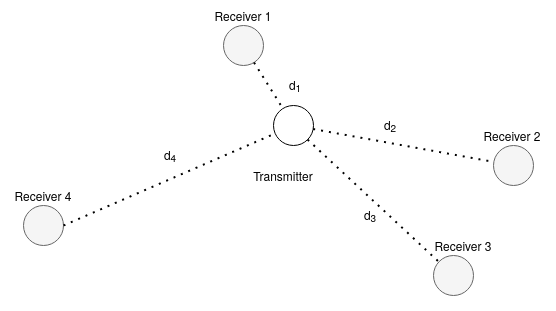
\includegraphics[width=\linewidth]{../Photos/tdoa-multiple.png}
      {(a) Single signal - multiple receivers}
    \end{minipage}%
    % -----------------
    \begin{minipage}{.5\textwidth}
      \centering
      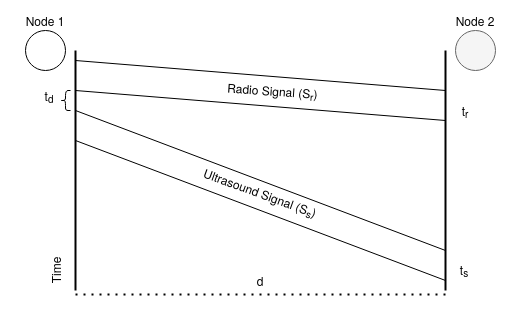
\includegraphics[width=\linewidth]{../Photos/tdoa-timing.png}
      {(b) Multiple signals - single receiver}
    \end{minipage}
    \hfill \break
    \decoRule
    \caption[Time Difference of Arrival cases]{Time Difference of Arrival cases}
    \label{fig:Time-Difference-of-Arrival-cases}
\end{figure}


Η πρώτη περίπτωση σχετίζεται με single signal και multiple receivers και παρουσιάζεται στο 
Figure \ref{fig:Time-Difference-of-Arrival-cases} (a), 
η οποία χρησιμοποιείται συνήθως στα cellular network και απαιτεί την ύπαρξη 
τουλάχιστον 4 beacons για τον υπολογισμό της θέσης ενός free node στον τρισδιάστατο χώρο. Υπολογίζει την χρονική διαφορά
που έφτασε σε καθένα από τα beacons το σήμα που έστειλε το free node, για τον υπολογισμό της απόστασης του free node από
το καθένα από αυτά. Σημαντικό σε αυτήν την περίπτωση είναι και εδώ, να είναι απόλυτα συγχρονισμένα τα beacons. 
Η γενική ιδέα σε αυτήν την περίπτωση περιγράφεται στην εξίσωση (\ref{eq:tdoa-multiple}) \cite{wsn-Localization-techniques} \cite{simple-tdoa} - και αυτό που 
θέλουμε, είναι να υπολογίσουμε την θέση του $r_t$ (free node) γνωρίζοντας για κάθε δύο διαφορετικά $r_i$ και $r_j$ beacon nodes
την χρονική στιγμή $t_i$ και $t_j$ που έφτασε το σήμα στο καθένα - εάν αυτό κινούταν με ταχύτητα s και το $\norm{\cdot}$ αναπαριστά την ευκλείδεια
απόσταση μεταξύ τους.

\begin{align}
	\Delta t_{ij} \triangleq & t_i - t_j = \frac{1}{s} (\norm{r_i - r_t} - \norm{r_j - r_t}), \quad i \neq j\label{eq:tdoa-multiple}
\end{align}

Η δεύτερη εκδοχή της χρήσης \hyperref[abbr:TDoA]{TDoA} - η οποία είναι πιο συχνή στα \hyperref[abbr:WSN]{WSN} και μας ενδιαφέρει περισσότερο, 
χρησιμοποιεί multiple signals με single receiver και παρουσιάζεται στο Figure \ref{fig:Time-Difference-of-Arrival-cases} (b). 
Αρχή λειτουργίας έχει ότι ο transmitter θα στείλει πολλαπλά διαφορετικού είδους σήματα και ο δέκτης θα μετρήσει την χρονική διαφορά 
που τα έλαβε. Ως παράδειγμα μπορεί το ένα σήμα να είναι σε \hyperref[abbr:RF]{RF} και να κινείται με ταχύτητα $s_r=c_o$ και το άλλο 
ηχητικό με ταχύτητα $s_s \approx 340m/s$. Αν $t_1$ τη χρονική στιγμή που λαμβάνει το \hyperref[abbr:RF]{RF} σήμα ενώ $t_2$ το ηχητικό,
μπορούμε να υπολογίσουμε την απόσταση μεταξύ των κόμβων από την εξίσωση (\ref{eq:tdoa-distance})
\cite{wsn-Localization-systems}.

\begin{align}
	d=&(s_r-s_s)(t_2-t_1) \label{eq:tdoa-distance}
\end{align}

Θετικό σε αυτήν την μέθοδο είναι ότι το error μπορεί να είναι της τάξης των μερικών εκατοστών, όμως αρχικά απαιτεί επιπλέον εξοπλισμό στο node -
ώστε να μπορεί να στείλει και να λάβει πολλαπλά είδη σήματος - πράγμα που μπορεί να το κάνει αντιοικονομικό ή αρκετά μεγαλύτερο σε διαστάσεις από 
το επιθυμητό. Όπως επίσης - και μάλιστα  
σημαντικότερο - η απόσταση η οποία μπορεί να 
χρησιμοποιηθεί, επηρεάζεται σε μεγάλο βαθμό από τα χαρακτηριστικά του δεύτερου σήματος. Ως παράδειγμα τα ηχητικά σήματα 
δεν μπορούν να μεταφερθούν σε μεγάλες αποστάσεις ή το ότι η ταχύτητα τους μπορεί να επηρεαστεί σημαντικά από περιβαλλοντολογικούς παράγοντες
\cite{farooqiazam2016location}.



%----------------------------------------------------------------------
% \subsubsection{Lighthouse}


%----------------------------------------------------------------------
\subsection{Angle}\label{sec:Chapter2-1-1}
Άλλη μία χρήσιμη μέτρηση η οποία μας ενδιαφέρει, είναι η εκτίμηση της γωνίας από την οποία λαμβάνουμε το σήμα ενός γειτονικού
node σε σχέση με έναν άξονας αναφοράς. Ο άξονας αυτός μπορεί να είναι είτε κοινώς για όλα τα nodes (π.χ. ως προς το βόρειο γεωγραφικό πόλο),
είτε μπορεί να είναι για το κάθε node ξεχωριστός, ως παράδειγμα με βάση τον προσανατολισμό του ίδιου του node ή με βάση την γωνία λήψης ενός 
επιπλέον σήματος \cite{wsn-Localization-systems}. Την πληροφορία αυτή την βρίσκουμε στην βιβλιογραφία να ονομάζεται Angle of Arrival 
(\hyperref[abbr:AoA]{AoA}) ή Direction of Arrival (\hyperref[abbr:DoA]{DoA}).

TODO: Angle of Arrival

%----------------------------------------------------------------------------------------
%	SECTION 2
%----------------------------------------------------------------------------------------
\section{Position Computation} \label{sec:Chapter2-2} 
Αν έχουμε δύο nodes, οι μετρήσεις που λάβαμε από το Section \ref{sec:Chapter2-1} είναι αρκετές για να γνωρίζουμε την θέση του καθενός,
συνεπώς ενδιαφέρον βρίσκεται στην ύπαρξη τριών ή παραπάνω nodes σε ένα σύστημα. Με βάση τις πληροφορίες που έχουμε συλλέξει - μέσω των τεχνικών που 
περιγράφτηκαν στο προηγούμενο κεφάλαιο - θα προσπαθήσουμε πλέον να εκτιμήσουμε την θέση ενός node. Στην συνέχεια αυτού του section περιγράφονται μέθοδοι οι οποίοι μπορούν να χρησιμοποιηθούν για να το επιτύχουν
αυτό. Κύρια διαφορά τους είναι η απόδοση που μπορεί να έχουν, η οποία όμως σχετίζεται με την αύξηση της πολυπλοκότητας στους υπολογισμούς που θα
χρειαστούν καθώς επίσης και ποιες από τις παραπάνω πληροφορίες θα εκμεταλλευτούν. 

Για την εύρεση της θέσης ενός unknown node στο τρισδιάστατο χώρο $(\mathfrak{R}^3)$ ως ελάχιστο χρειαζόμαστε τέσσερα επιπλέον nodes.
Στις παρακάτω περιγραφές όμως, και χωρίς βλάβη της γενικότητας θα χρησιμοποιηθούν τρία για την απλούστευση της περιγραφής, με την παραδοχή ότι μας
ενδιαφέρει η δισδιάστατη ανάλυση $(\mathfrak{R}^2)$.

\begin{figure} [H]
	\centering
	
    % -----------------
		\begin{minipage}{.33\textwidth}
			\centering
			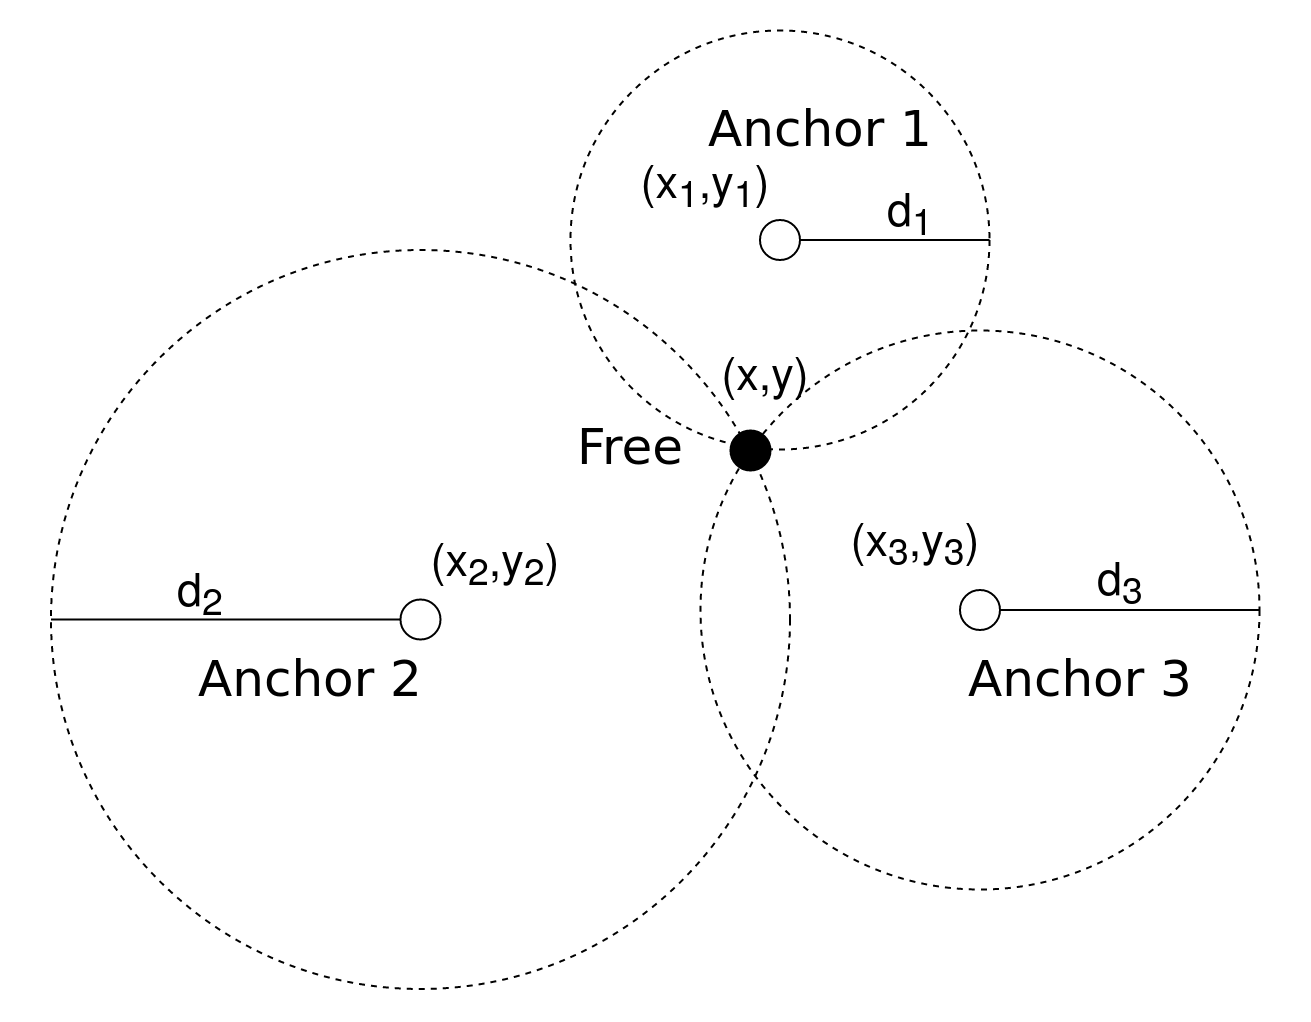
\includegraphics[width=\linewidth]{../Photos/Trilateration-ideal.png}
			{(a) Ideal Trilateration}
		\end{minipage}%
		% -----------------
		\begin{minipage}{.33\textwidth}
			\centering
			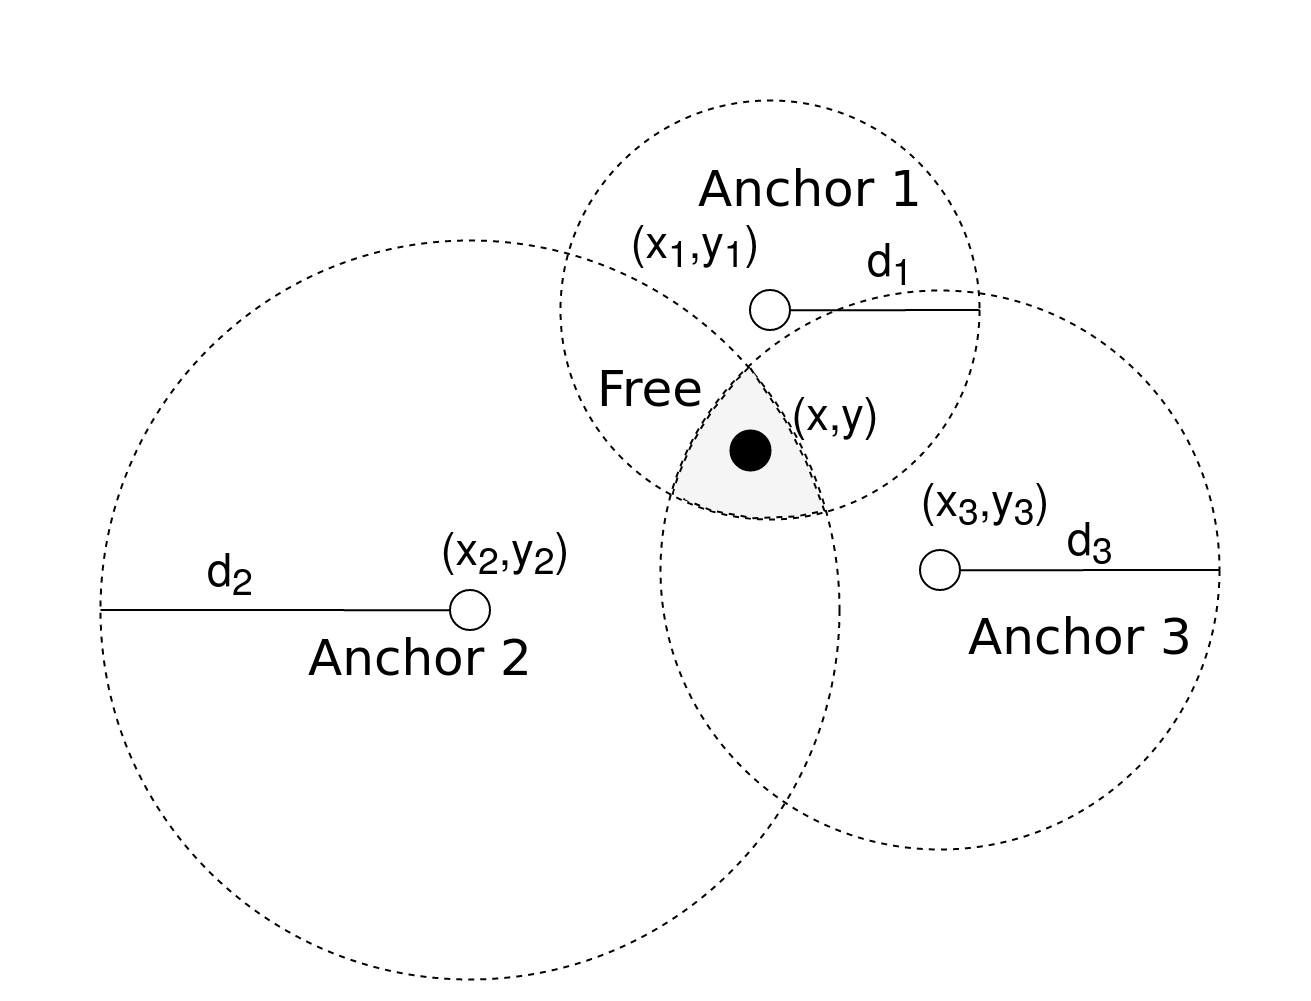
\includegraphics[width=\linewidth]{../Photos/Trilateration-actual.png}
			{(b) Realistic Trilateration}
		\end{minipage}
		% -----------------
		\begin{minipage}{.33\textwidth}
			\centering
			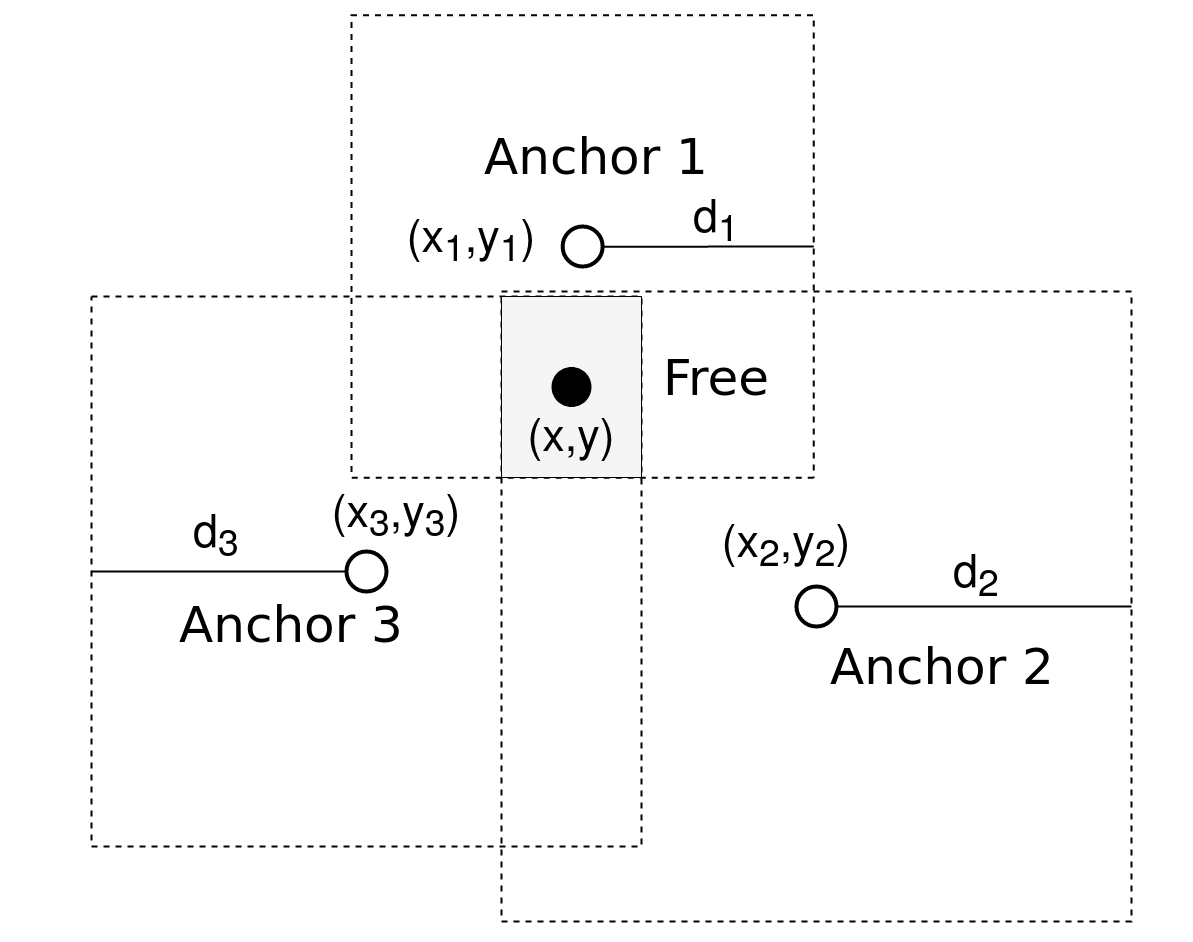
\includegraphics[width=\linewidth]{../Photos/Bounding-box.png}\\
			{(c) Bounding Box}
		\end{minipage}
	% -----------------
    \hfill \break
    \decoRule
    \caption[Position Computation using distance]{Position Computation using distance}
    \label{fig:Position-Computation-using-distance}
\end{figure}

%----------------------------------------------------------------------
\subsubsection{Trilateration}
Η συγκεκριμένη μέθοδος είναι ίσως η πιο απλή διαισθητικά, βασίζεται στην γεωμετρία κύκλων, είναι αυτή που χρησιμοποιείται από τα \hyperref[abbr:GPS]{GPS}
για τον υπολογισμό θέσης \cite{trilateration-vs-triangulation-video}, ενώ αξιοποιεί μόνο πληροφορία απόστασης και όχι γωνίας \cite{Trilateration-vs-Triangulation}.
Η εξίσωση ενός κύκλου από την γεωμετρία γνωρίζουμε ότι περιγράφεται από την εξίσωση (\ref{eq:trilateration-circles}) όπου $(x_i,y_i)$ οι συντεταγμένες
του κέντρο του κύκλου με ακτίνα $d_i$.

\begin{align}
	(x-x_i)^2 + (y-y_i)^2 &= d_i^2 \label{eq:trilateration-circles}
\end{align}

Εάν χρησιμοποιούμε omnidirectional κεραίες \cite{Omnidirectional-antenna} ή στην γενικότερη περίπτωση το μοντέλο της isotropic antenna \cite{Isotropic-radiator} και υπολογίσουμε την απόσταση ενός beacon από το node στο οποίο θέλουμε να υπολογίσουμε την θέση του -
τότε μπορούμε να συμπεράνουμε ότι το free node είναι κάπου πάνω στην περιφέρεια ενός 
κύκλου, με κέντρο το beacon και ακτίνα την απόσταση μεταξύ του beacon και του free node. 
Επαναλαμβάνοντας αυτό για ακόμα δύο beacons, τελικά το free node στο δισδιάστατο επίπεδο $(\mathfrak{R}^2)$ θα πρέπει να βρίσκεται στην τομή των τριών κύκλων, πράγμα που γραφικά 
απεικονίζεται στο Figure \ref{fig:Position-Computation-using-distance} (a) \cite{RSSI-trilateration-Range_based}.

\begin{align}
	x^2-2 x_1 x + x_1^2 + y^2-2 y_1 y + y_1^2 &= d_1^2 \label{eq:trilateration-b1} \\ 
	x^2-2 x_2 x + x_2^2 + y^2-2 y_2 y + y_2^2 &= d_2^2 \label{eq:trilateration-b2} \\
	x^2-2 x_3 x + x_3^2 + y^2-2 y_3 y + y_3^2 &= d_3^2 \label{eq:trilateration-b3} 
\end{align}

Οι εξισώσεις (\ref{eq:trilateration-b1}), (\ref{eq:trilateration-b2}) και (\ref{eq:trilateration-b3}) περιγράφουν πλήρως τους κύκλους του κάθε node από το παράδειγμα 
του Figure \ref{fig:Position-Computation-using-distance} (a),
όπου $(x_i,y_i)$ το κέντρο του κύκλου, $d_i$ η ακτίνα του - για κάθε beacon $i=1,2,3$ και τελικά $(x,y)$ οι συντεταγμένες του free nodes τις οποίες και ψάχνουμε. 
Ένας τρόπος να υπολογίσουμε τις συντεταγμένες αυτές είναι να αφαιρέσουμε από την (\ref{eq:trilateration-b2}) την (\ref{eq:trilateration-b1}) και όμοια από την 
(\ref{eq:trilateration-b3}) την (\ref{eq:trilateration-b2}) ώστε να καταλήξουμε στις παρακάτω δύο εξισώσεις \cite{trilateration-equations} \cite{localization-algorithms-for-wsn}.

\begin{align}
	(-2x_1+2x_2)x + (-2y_1+2y_2)y = d_1^2 - d_2^2 - x_1^2 + x_2^2 - y_1^2 + y_2^2  \nonumber \\
	(-2x_2+2x_3)x + (-2y_2+2y_3)y = d_2^2 - d_3^2 - x_2^2 + x_3^2 - y_2^2 + y_3^2  \nonumber
\end{align}

Ο λόγος που κάναμε το παραπάνω βήμα είναι διότι πλέον έχουμε ένα σύστημα με δύο εξισώσεις και δύο αγνώστους, οπότε μπορούμε εύκολα να θεωρήσουμε τους παρακάτω πίνακες.

\begin{align}
	A = \begin{bmatrix} -2x_1+2x_2 & -2y_1+2y_2 \\ -2x_2+2x_3 & -2y_2+2y_3 \end{bmatrix} \nonumber \quad
	X = \begin{bmatrix} x \\ y \end{bmatrix} \nonumber \quad
	B = \begin{bmatrix} d_1^2 - d_2^2 - x_1^2 + x_2^2 - y_1^2 + y_2^2 \\ d_2^2 - d_3^2 - x_2^2 + x_3^2 - y_2^2 + y_3^2 \end{bmatrix} \nonumber
\end{align}

Με την χρήση των οποίων καταλήγουμε ότι έχουμε να λύσουμε το γραμμικό σύστημα πινάκων που περιγράφεται από την εξίσωση (\ref{eq:trilateration-linear-system}) για τον
υπολογισμό των συντεταγμένων $(x,y)$ του free node οι οποίες μας ενδιαφέρουν.

\begin{align}
	AX = B \label{eq:trilateration-linear-system}
\end{align}

Όπως αναφέρθηκε και στις προηγούμενες ενότητες, ο υπολογισμός της απόστασης πολύ πιθανόν να περιλαμβάνει μια μικρή απόκλιση $\widehat{d_i} = d_i - ε$, 
με το ε συχνά να θεωρείται μία ανεξάρτητη κανονική τυχαία μεταβλητή με μηδενικό μέσο. Αυτό σημαίνει ότι
τότε οι κύκλοι δεν έχουν ένα κοινό σημείο τομής, αλλά το free node βρίσκεται κάπου μέσα στο χωρίο επικάλυψης
των τριών κύκλων, σχηματικά αυτό παρουσιάζεται στο Figure \ref{fig:Position-Computation-using-distance} (b) και σε αυτήν την περίπτωση καταλήγουμε σε ένα
μη πεπερασμένο πλήθος λύσεων, με τη συνάρτηση του κάθε κύκλου να περιγράφεται από την εξίσωση
(\ref{eq:trilateration-circles-error}) \cite{wsn-Localization-systems}.

\begin{align}
	(x-x_i)^2 + (y-y_i)^2 &= d_i^2-e \label{eq:trilateration-circles-error}
\end{align}

Το αρνητικό με αυτήν την μέθοδο, είναι η ανάγκη πραγματοποίησης floating point operations για τον υπολογισμό των συντεταγμένων $(x,y)$ σε πραγματικές συνθήκες - όπου το πλήθος
των οποίων εξαρτάται από τον τρόπο που θα επιλέξουμε να επιλύσουμε το σύστημα. 
Ένας από της μεθόδους επίλυσης της γραμμικής εξίσωσης είναι μέσω του least square method, όπου τότε το πλήθος των floating point operations
που απαιτούνται είναι $(m+n/3)n^2$ με $m$ τον αριθμό των αγνώστων και $n$ τον αριθμό των δοθέντων εξισώσεων \cite{wsn-Localization-systems}.

%----------------------------------------------------------------------
\subsubsection{Bounding Box}
Σε αυτήν την μέθοδο χρησιμοποιούνται τετράγωνα αντί για κύκλους του Trilateration, ενώ και εδώ θεωρούμε $(x_i,y_i)$
τις συντεταγμένες των beacon και $d_i$ η απόσταση που έχουμε υπολογίσει από το free node - για κάθε beacon $i$. Δημιουργούμε
τετράγωνα μήκος πλευράς $2d_i$ με κέντρο το κέντρο του beacon και συντεταγμένες $(x_i - d_i, y_i - d_i)$ \& $(x_i + d_i, y_i + d_i)$. 
Θετικό πλέον είναι ότι δεν χρειάζεται να κάνουμε floating point operations για τον υπολογισμό του χωρίου τομής - αλλά μπορούμε να το υπολογίσουμε
με απλή γεωμετρία. Αφού έχουμε υπολογίσει το χωρίο τομής των τετραγώνων μπορούμε να θεωρήσουμε ότι στο κέντρο του βρίσκεται το free node.
Παράδειγμα αυτής της μεθόδου βρίσκεται στο Figure \ref{fig:Position-Computation-using-distance} (c).
Η συγκεκριμένη μέθοδος μπορεί να είναι ευκολότερη υπολογιστικά και να απαιτεί λιγότερα processor resources από το Trilateration, όμως ταυτόχρονα 
προκύπτει και μεγαλύτερο σφάλμα απόκλισης \cite{wsn-Localization-systems}.   

%----------------------------------------------------------------------
\subsubsection{Triangulation}
Σε αντίθεση με τις παραπάνω μεθόδους, η τεχνική Triangulation εκτιμάει την θέση του node που μας ενδιαφέρει, χρησιμοποιώντας   

%----------------------------------------------------------------------
\subsubsection{Multilateration}

%----------------------------------------------------------------------
\subsubsection{Probabilistic approaches}


%----------------------------------------------------------------------------------------
%	SECTION 3
%----------------------------------------------------------------------------------------
\section{Localization Algorithm} \label{sec:Chapter2-3} 

%----------------------------------------------------------------------
\subsubsection{Range-based vs Range-free}

%----------------------------------------------------------------------
\subsubsection{Distributed vs Centralized Position Computation}

%----------------------------------------------------------------------
\subsubsection{Relative vs Absolute Positioning}

%----------------------------------------------------------------------
\subsubsection{Indoor vs Outdoor}

%----------------------------------------------------------------------
\subsubsection{One-hop vs Multihop}

%----------------------------------------------------------------------
\subsubsection{With vs Without Infrastructure}
